\documentclass[conference]{IEEEtran}
\IEEEoverridecommandlockouts
% The preceding line is only needed to identify funding in the first footnote. If that is unneeded, please comment it out.
%Template version as of 6/27/2024

\usepackage{cite}
\usepackage{amsmath,amssymb,amsfonts}
\usepackage{algorithmic}
\usepackage{graphicx}
\usepackage{textcomp}
\usepackage{xcolor}
\def\BibTeX{{\rm B\kern-.05em{\sc i\kern-.025em b}\kern-.08em
    T\kern-.1667em\lower.7ex\hbox{E}\kern-.125emX}}
\begin{document}

\title{Line-of-Sight Analysis for Urban Free-Space Optical Communication\\}

\author{\IEEEauthorblockN{1\textsuperscript{st} Leonard Nolting}
\IEEEauthorblockA{
    \textit{Chair of Communication Networks} \\
    \textit{Technical University of Munich}\\
    Munich, Germany \\
    leonard.nolting@tum.de}
\and
\IEEEauthorblockN{2\textsuperscript{nd} Kevin Jiokeng}
\IEEEauthorblockA{\textit{Laboratoire d'Informatique} \\
\textit{École Polytechnique}\\
Palaiseau, France \\
kevin.jiokeng@polytechnique.edu}
\and
\IEEEauthorblockN{3\textsuperscript{rd} Hansini Vijayaraghavan}
\IEEEauthorblockA{\textit{Chair of Communication Networks} \\
\textit{Technical University of Munich}\\
Munich, Germany \\
hansini.vijayaraghavan@tum.de}
\and
\IEEEauthorblockN{4\textsuperscript{th} Juan-Antonio Cordero-Fuertes}
\IEEEauthorblockA{\textit{Laboratoire d'Informatique} \\
\textit{École Polytechnique}\\
Palaiseau, France \\
juan-antonio.cordero-fuertes@polytechnique.edu}
}

\maketitle

\begin{abstract}
This document is a model and instructions for \LaTeX.
This and the IEEEtran.cls file define the components of your paper [title, text, heads, etc.]. *CRITICAL: Do Not Use Symbols, Special Characters, Footnotes, 
or Math in Paper Title or Abstract.
\end{abstract}

\begin{IEEEkeywords}
Free-Space Optical Communication (FSO), mobile networks, backhaul, line-of-sight (LoS)
\end{IEEEkeywords}

\section{Introduction}\label{sec:introduction}

\begin{figure}[htbp]
    \centerline{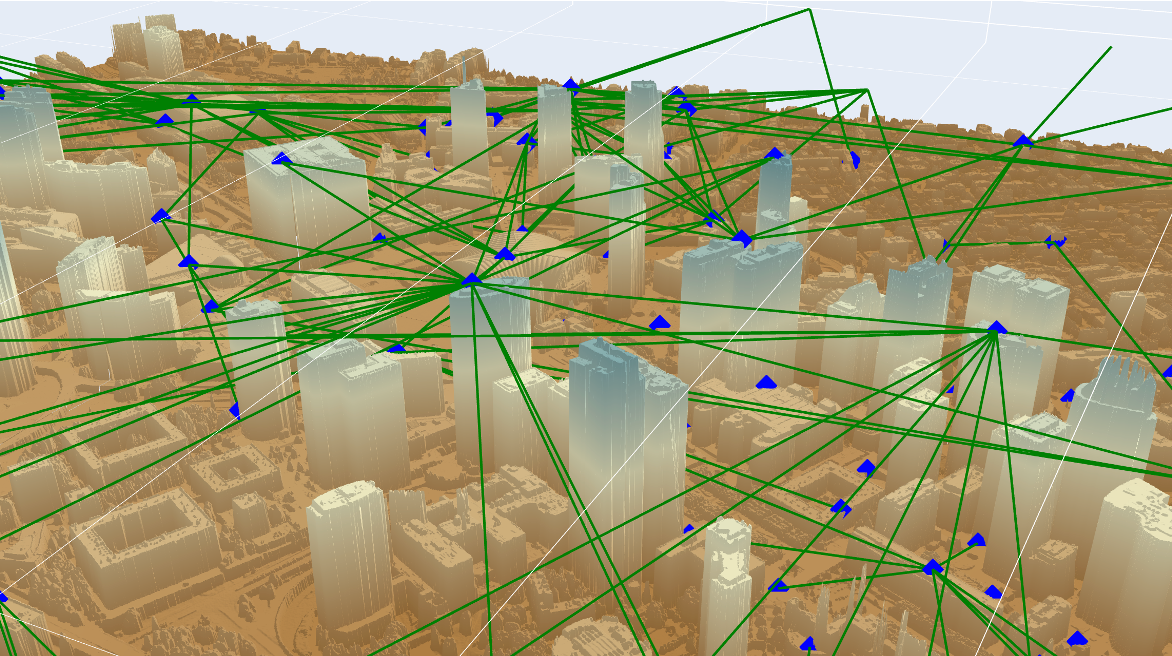
\includegraphics[width=\columnwidth]{figures/scenario}}
    \caption{Clear lines-of-sight for an urban FSO network.}
    \label{fig:scenario}
\end{figure}

Free-Space Optics (FSO) is a technology that uses light beams for wireless point-to-point communication through air.
It offers fiber-like bandwidths without the trenching/leasing costs or spectrum licensing fees typically associated with wired alternatives and radio frequency alternatives, respectively~\cite{urbanfsosurvey}.
While experiments show terabit-speeds over many kilometers on earth~\cite{fastfsozurich, fastfsourban, fastfsojapan} and through the solar system in space~\cite{nasaspace}, the unguided channel limits data rate and link length during weather conditions that scatter and refract the light, such as fog, rain and turbulence~\cite{systematicsurvey}.
Simulations have to focus on the worst-case conditions to guarantee high availability, crucial for consistent QoS and QoE~\cite{outageqoe}.
Relaying traffic at several intermediate hops mitigates the problem by splitting long paths up into shorter ones that withstand adverse conditions better~\cite{relays, hybridfso}.
Urban networks may, as a consequence, due to their dense mesh nature, emerge as a natural fit for highly available FSO networks.
Besides the best-case bandwidths and lack of trenching and spectrum license costs, a mesh FSO deployment comes with several other anticipated advantages.
High redundancy to more hierarchical topologies has the potential to protect against momentary and equipment outages, e.g.,\ from momentary obstructions in the line-of-sight like birds, or power loss of a relay~\cite{fsomeshsurvey}.
The wireless and license-free nature allows for flexible and rapid deployment.
Systems can be ``operative within hours'' and have acted as spontaneous backup links during disasters or irregular events~\cite{urbanfsosurvey}.
In contrast to high upfront costs of laying fiber, an FSO mesh can be deployed gradually, decreasing capital expenditures~\cite{fiberwithoutfiber}.
As average link length shrinks at higher density, we will see that the network benefits from scaling in density, potentially promoting Fixed Wireless Access and reusing the FSO infrastructure for both Cellular Backhaul and Last Mile (``FSO To The Building'').
Removing the wire reduces the risk for an entire class of vulnerabilities, such as excavation accidents, landslides and earthquakes~\cite{fsodigging, fibervulnerability}.

FSO has a research history dating back to 1880~\cite{fsosurveydefault}.
Many of the hard engineering challenges have been ``solved in the past three decades''~\cite{invited}, but some challenges, especially specific to the urban environment, remain: Eye safety regulations vary by country, but may limit transmission power, building sway adds beam alignment complexity, and heat shimmer above hot roofs causes signal scintillation~\cite{urbanfsosurvey, fsobackhaul}.

One of the biggest remaining obstacles for urban FSO, however, originates from the point-to-point nature of FSO links: A line-of-sight must exist between transmitter and receiver~\cite{systematicsurvey}.

\subsection*{Contributions}\label{subsec:contributions}

In this thesis, we develop and implement a method to check individual lines for line-of-sight availability.

Our goal is to analyze the topology of urban networks created purely from verified lines-of-sight.

As link ranges that can be sustained are limited during worst case conditions, we will provide network connectivity metrics over topologies that deploy only links up to a variable maximum length.
From that data, we can derive values that suggest what link ranges need to be supported for various degrees of connectivity in urban FSO networks.
This data can also aid in the judgment which priority needs to be given to the FSO line-of-sight requirement during selection of node locations (for example, as opposed to cellular coverage or cost), or in an extreme case, how well FSO can be retrofitted to existing sites and what role additional mirrors and relays play.

Data rate and capacity simulations are out of the scope of this work, but can build on this work by selecting a set of gateway locations, which connect the FSO network to the internet backbone, and simulating traffic flows from the edge to the gateways.

As a sample dataset for an urban network, we choose an official database of cell sites, simulating a mobile backhaul backbone.
We ran the simulation for 19 million lines in the greater Paris area and find that in a topology of links of up to one kilometer length, 91\% of the considered nodes have at least one line-of-sight.
Moreover, increasing link length beyond around one kilometer has diminishing returns in increased connectivity, but vastly increases options for redundancy and reduces the average hop count between nodes.
At 300 m, a single connected component emerges covering the city of Paris, with 95.8\% of nodes in the region covered by its concave hull connected to the component.

maybe: Short lines (due to worst-case assumption) aid line-of-sight availability.

maybe: Small world: Hop count can be reduced during good conditions

\subsection*{Related Work}\label{subsec:related-work}
weather link ranges: commonly studied → cite values for ballpark idea (100-500 m) (later contrast: we look at what is necessary)

relays: also widely accepted as a very, if not the most effective counter-measurement

line-of-sight: obstructions usually LoD 1, e. g. FSONet (later contrast: LiDAR far more detailed)

\subsection*{Contributions}\label{subsec:contributions2}
Close to existing contributions chapter

- What do we do, raw
    - Allude to relay idea from introduction (hop by hop)
    - worst-case analysis (short links - reader will think "many"?); briefly cut on optimizations for average-cases, regarding hop counts (relieve reader: not many hops usually), and fault resilience briefly
    - take ideas from presentation for a logical introduction to our methodology
    - Be very clear about what we do not do, too (capacities, gateways, TE, ...)
- Contrast to Related Work:
    - Derive required link lengths from reality of mesh density
    - Use more accurate obstruction models (only tease here, this is our transition to sec:implementation)

\subsection*{Paper Outline}\label{subsec:structure}
We continue by introducing our implementation for line-of-sight analysis, including data source selection, preprocessing steps, a comparison of ray tracing algorithms, and a note on adapting this implementation to different geographic areas and cell site locations.

... evaluation ...

... validation ...

... conclusion ...

% No background chapter (FSO background is briefly introduced in introduction - "what is FSO and its main challenge")

\section{Implementation}\label{sec:implementation}
explain that links = between nodes => only need nodes

cell sites source? → country: France
preprocessing - snapping and filtering

Simulating realistic lines-of-sight requires a model of obstructions of the world.
- Statistical models (Manhattan grid)
- OpenStreetMap building footprints + height = LoD1
- Commercial options exist which offer increased accuracy based on LiDAR measurements, as well as raw LiDAR point clouds, post-processed formats thereof and multi-sensor measurements. Pricing models? (subscription; root tile request for 3h; not disclosed)
- since nodes from France, what about specifically in France?
- France public option LiDAR HD: open / free access, good nationwide coverage, high accuracy
- France also: processed format DSMs. explain DSMs. good compromise for us: standardized, simple format (2D array), easy to manage (lower storage), cell sites generally high (not underneath obstructions)

Conceptually, computing collisions of a line with the obstruction model requires calculating which pixels of the DSM raster it crosses and checking if the surface at any of those pixels is higher than the line.

Line rasterization algorithms from computer graphics, such as Bresenham's and Xiaolin Wu's algorithm, solve a similar problem of painting pixels between two lines [TODO quote].
Designed for another purpose, however, they do not paint exactly all pixels touched by the line, skipping over potential obstacles [TODO show? figure? or good without deeper explanation?].
Sampling points along the line at a rate of two samples per pixel shows accuracy gains at similar speeds, but still misses pixels.
The Python library rasterio offers a function masking exactly all pixels touched by a line, which in turn calls to GDAL [TODO quote].
Tests show the fastest accurate CPU-based method to be ``A Fast Voxel Traversal Algorithm'' by Amanatides and Woo [TODO quote].
... CUDA ...

NVIDIA and other graphics processing unit producers offer dedicated ray tracing offloading cores and SDKs. For instance, NVIDIA RTX GPUs can be programmed with the OptiX SDK by building a BVH (bounding volume hierarchy) acceleration structure (AS) in memory and running line-of-sight checks against that almost entirely in hardware.
Our tests show that the main bottleneck becomes the memory transfer of the DSM to the accelerator, the time spent on building the AS and the additional memory occupied by the AS.
The DSM can be seen as a two-dimensional grid of ``pixel pillars'' - each pixel a cuboid stretching from -inf to the surface height at the pixel.
Converting the DSM to triangle primitives without quality loss requires two triangles per visible surface, which are laid out as one rectangle.
Since the top surface of a pixel is always visible, and the bottom pixel is always covered by the sides of this and neighboring pixels and is never visible, and assuming that on average two sides are visible per pixel, this results in six triangles per pixel.
... 3 floats per triangle, 1 after compaction, too many values, memory inflation ...
Using instance acceleration structures (IAS), which allow replicating one AS by shifting and scaling it, may reduce this memory inflation.
NVIDIA supports custom primitives for its ray tracing platform for any objects that cannot be modeled adequately with triangles.
Custom primitives assign an axis-aligned bounding box (AABB) containing the primitive and a custom shader, which will be invoked when a ray intersects the AABB. The ray tracing check is still offloaded and only hands over to the shader for an intersection with the AABB.
Since aforementioned ``pixel pillars'' are AABBs, they can be transformed to custom primitives.
Whenever the intersection shader is called, it already marks an intersection without further computation, and the line can immediately be marked as blocked.
Memory inflation can also be combated by smoothing out the model creating a triangulated RSG (regular square grid).
Each pixel is converted to one triangle that
... conservative conversion (always the maximum) ...
... performance: 6-8 gigarays per second for one 1*1km tile, but lines have to split up over tiles because AS cannot grow much larger ...
TODO: mention more explicitly that the CPU version generally is line-bound, whereas the RT version is area-bound

The choice of implementation between CPU, CUDA and OptiX depends primarily on the size of the datasets and region considered, the density of lines per area, implementation complexity and hardware accelerator availability.
For the data and area considered in this paper, the CPU version has sufficient performance, but derived work with significantly more lines to check will benefit from a hardware ray-traced version.

\subsection*{Adaptability}\label{subsec:adaptability}


\section{Evaluation}\label{sec:evaluation}
- Where exactly did we run our simulations (parameters)

- Walk through results, logical steps
    - data shows, as expected, short links are less obstructed; and as expected, there are more long candidate links ⇒ What is the distribution like?
    - do at least all nodes have one LoS?
        - 200m = majority
        - 300m = 3/4
        - >1000m = diminishing returns
    - urban → more dense → look at urban nodes specifically?
    - one LoS = one hop, but not entire path to other nodes; connected components?
        - 300m = big connected component
        - ...
    - path may exist, but at what cost? hop counts
    - reconfiguration, small world
    - fault resilience
        - redundancy per node? degrees
        - angular diversity (easily blocked by a new building or not?)
        - k-connectivity
        - structural hole analysis

TODO: how to integrate results of different cities (depends on what the results look like in the first place)
TODO: how to integrate results for different operators
TODO: how to integrate fault analysis results

\section{Validation}\label{sec:validation}
Why is what we do correct and what are the limitations?

... cell site locations ... (height: compared to Google Maps 3D, which itself may not be perfect)

... lidar data ... (both methodologically and accuracy)

... implementation ... (earth's curvature + atmospheric refraction, coordinate conversions, floating point?)

\section{Conclusion}\label{sec:conclusion}
Pick measured values back up from Related Work, and put in relation to our results (same as parts of ch:discussion from thesis)

-> What does this mean for the future?

And why is that relevant?

And why are these results credible?

(And how can we go on from here? Immediate next steps? How to form this into a meaningful framework?)

\vspace{12pt} % Keep?


\bibliographystyle{IEEEtran}
\bibliography{IEEEabrv,IEEEexample}

\end{document}
